
%% bare_jrnl.tex
%% V1.3
%% 2007/01/11
%% by Michael Shell
%% see http://www.michaelshell.org/
%% for current contact information.
%%
%% This is a skeleton file demonstrating the use of IEEEtran.cls
%% (requires IEEEtran.cls version 1.7 or later) with an IEEE journal paper.
%%
%% Support sites:
%% http://www.michaelshell.org/tex/ieeetran/
%% http://www.ctan.org/tex-archive/macros/latex/contrib/IEEEtran/
%% and
%% http://www.ieee.org/



% *** Authors should verify (and, if needed, correct) their LaTeX system  ***
% *** with the testflow diagnostic prior to trusting their LaTeX platform ***
% *** with production work. IEEE's font choices can trigger bugs that do  ***
% *** not appear when using other class files.                            ***
% The testflow support page is at:
% http://www.michaelshell.org/tex/testflow/


%%*************************************************************************
%% Legal Notice:
%% This code is offered as-is without any warranty either expressed or
%% implied; without even the implied warranty of MERCHANTABILITY or
%% FITNESS FOR A PARTICULAR PURPOSE! 
%% User assumes all risk.
%% In no event shall IEEE or any contributor to this code be liable for
%% any damages or losses, including, but not limited to, incidental,
%% consequential, or any other damages, resulting from the use or misuse
%% of any information contained here.
%%
%% All comments are the opinions of their respective authors and are not
%% necessarily endorsed by the IEEE.
%%
%% This work is distributed under the LaTeX Project Public License (LPPL)
%% ( http://www.latex-project.org/ ) version 1.3, and may be freely used,
%% distributed and modified. A copy of the LPPL, version 1.3, is included
%% in the base LaTeX documentation of all distributions of LaTeX released
%% 2003/12/01 or later.
%% Retain all contribution notices and credits.
%% ** Modified files should be clearly indicated as such, including  **
%% ** renaming them and changing author support contact information. **
%%
%% File list of work: IEEEtran.cls, IEEEtran_HOWTO.pdf, bare_adv.tex,
%%                    bare_conf.tex, bare_jrnl.tex, bare_jrnl_compsoc.tex
%%*************************************************************************

% Note that the a4paper option is mainly intended so that authors in
% countries using A4 can easily print to A4 and see how their papers will
% look in print - the typesetting of the document will not typically be
% affected with changes in paper size (but the bottom and side margins will).
% Use the testflow package mentioned above to verify correct handling of
% both paper sizes by the user's LaTeX system.
%
% Also note that the "draftcls" or "draftclsnofoot", not "draft", option
% should be used if it is desired that the figures are to be displayed in
% draft mode.
%
\documentclass[journal]{IEEEtran}
\usepackage{blindtext}
\usepackage{graphicx}
\usepackage{float}
\usepackage[T1]{fontenc}
\usepackage{csvsimple}


\usepackage{listings}
\usepackage{color}

\definecolor{mygreen}{rgb}{0,0.6,0}
\definecolor{mygray}{rgb}{0.5,0.5,0.5}
\definecolor{mymauve}{rgb}{0.58,0,0.82}

\lstset{ %
  backgroundcolor=\color{white},   % choose the background color; you must add \usepackage{color} or \usepackage{xcolor}
  basicstyle=\footnotesize,        % the size of the fonts that are used for the code
  breakatwhitespace=false,         % sets if automatic breaks should only happen at whitespace
  breaklines=true,                 % sets automatic line breaking
  captionpos=b,                    % sets the caption-position to bottom
  commentstyle=\color{mygreen},    % comment style
  deletekeywords={...},            % if you want to delete keywords from the given language
  escapeinside={\%*}{*)},          % if you want to add LaTeX within your code
  extendedchars=true,              % lets you use non-ASCII characters; for 8-bits encodings only, does not work with UTF-8
  frame=single,	                   % adds a frame around the code
  keepspaces=true,                 % keeps spaces in text, useful for keeping indentation of code (possibly needs columns=flexible)
  keywordstyle=\color{blue},       % keyword style
  language=Octave,                 % the language of the code
  otherkeywords={*,...},           % if you want to add more keywords to the set
  numbers=left,                    % where to put the line-numbers; possible values are (none, left, right)
  numbersep=5pt,                   % how far the line-numbers are from the code
  numberstyle=\tiny\color{mygray}, % the style that is used for the line-numbers
  rulecolor=\color{black},         % if not set, the frame-color may be changed on line-breaks within not-black text (e.g. comments (green here))
  showspaces=false,                % show spaces everywhere adding particular underscores; it overrides 'showstringspaces'
  showstringspaces=false,          % underline spaces within strings only
  showtabs=false,                  % show tabs within strings adding particular underscores
  stepnumber=1,                    % the step between two line-numbers. If it's 1, each line will be numbered
  stringstyle=\color{mymauve},     % string literal style
  tabsize=2,	                   % sets default tabsize to 2 spaces
  title=\lstname                   % show the filename of files included with \lstinputlisting; also try caption instead of title
}

% Some very useful LaTeX packages include:
% (uncomment the ones you want to load)


% *** MISC UTILITY PACKAGES ***
%
%\usepackage{ifpdf}
% Heiko Oberdiek's ifpdf.sty is very useful if you need conditional
% compilation based on whether the output is pdf or dvi.
% usage:
% \ifpdf
%   % pdf code
% \else
%   % dvi code
% \fi
% The latest version of ifpdf.sty can be obtained from:
% http://www.ctan.org/tex-archive/macros/latex/contrib/oberdiek/
% Also, note that IEEEtran.cls V1.7 and later provides a builtin
% \ifCLASSINFOpdf conditional that works the same way.
% When switching from latex to pdflatex and vice-versa, the compiler may
% have to be run twice to clear warning/error messages.






% *** CITATION PACKAGES ***
%
%\usepackage{cite}
% cite.sty was written by Donald Arseneau
% V1.6 and later of IEEEtran pre-defines the format of the cite.sty package
% \cite{} output to follow that of IEEE. Loading the cite package will
% result in citation numbers being automatically sorted and properly
% "compressed/ranged". e.g., [1], [9], [2], [7], [5], [6] without using
% cite.sty will become [1], [2], [5]--[7], [9] using cite.sty. cite.sty's
% \cite will automatically add leading space, if needed. Use cite.sty's
% noadjust option (cite.sty V3.8 and later) if you want to turn this off.
% cite.sty is already installed on most LaTeX systems. Be sure and use
% version 4.0 (2003-05-27) and later if using hyperref.sty. cite.sty does
% not currently provide for hyperlinked citations.
% The latest version can be obtained at:
% http://www.ctan.org/tex-archive/macros/latex/contrib/cite/
% The documentation is contained in the cite.sty file itself.






% *** GRAPHICS RELATED PACKAGES ***
%
\ifCLASSINFOpdf
  % \usepackage[pdftex]{graphicx}
  % declare the path(s) where your graphic files are
  % \graphicspath{{../pdf/}{../jpeg/}}
  % and their extensions so you won't have to specify these with
  % every instance of \includegraphics
  % \DeclareGraphicsExtensions{.pdf,.jpeg,.png}
\else
  % or other class option (dvipsone, dvipdf, if not using dvips). graphicx
  % will default to the driver specified in the system graphics.cfg if no
  % driver is specified.
  % \usepackage[dvips]{graphicx}
  % declare the path(s) where your graphic files are
  % \graphicspath{{../eps/}}
  % and their extensions so you won't have to specify these with
  % every instance of \includegraphics
  % \DeclareGraphicsExtensions{.eps}
\fi
% graphicx was written by David Carlisle and Sebastian Rahtz. It is
% required if you want graphics, photos, etc. graphicx.sty is already
% installed on most LaTeX systems. The latest version and documentation can
% be obtained at: 
% http://www.ctan.org/tex-archive/macros/latex/required/graphics/
% Another good source of documentation is "Using Imported Graphics in
% LaTeX2e" by Keith Reckdahl which can be found as epslatex.ps or
% epslatex.pdf at: http://www.ctan.org/tex-archive/info/
%
% latex, and pdflatex in dvi mode, support graphics in encapsulated
% postscript (.eps) format. pdflatex in pdf mode supports graphics
% in .pdf, .jpeg, .png and .mps (metapost) formats. Users should ensure
% that all non-photo figures use a vector format (.eps, .pdf, .mps) and
% not a bitmapped formats (.jpeg, .png). IEEE frowns on bitmapped formats
% which can result in "jaggedy"/blurry rendering of lines and letters as
% well as large increases in file sizes.
%
% You can find documentation about the pdfTeX application at:
% http://www.tug.org/applications/pdftex


%URL package for url links in the bibliography
\usepackage{url}


% *** MATH PACKAGES ***
%
\usepackage[cmex10]{amsmath}
\usepackage{bm}
% A popular package from the American Mathematical Society that provides
% many useful and powerful commands for dealing with mathematics. If using
% it, be sure to load this package with the cmex10 option to ensure that
% only type 1 fonts will utilized at all point sizes. Without this option,
% it is possible that some math symbols, particularly those within
% footnotes, will be rendered in bitmap form which will result in a
% document that can not be IEEE Xplore compliant!
%
% Also, note that the amsmath package sets \interdisplaylinepenalty to 10000
% thus preventing page breaks from occurring within multiline equations. Use:
\interdisplaylinepenalty=2500
% after loading amsmath to restore such page breaks as IEEEtran.cls normally
% does. amsmath.sty is already installed on most LaTeX systems. The latest
% version and documentation can be obtained at:
% http://www.ctan.org/tex-archive/macros/latex/required/amslatex/math/





% *** SPECIALIZED LIST PACKAGES ***
%
%\usepackage{algorithmic}
% algorithmic.sty was written by Peter Williams and Rogerio Brito.
% This package provides an algorithmic environment fo describing algorithms.
% You can use the algorithmic environment in-text or within a figure
% environment to provide for a floating algorithm. Do NOT use the algorithm
% floating environment provided by algorithm.sty (by the same authors) or
% algorithm2e.sty (by Christophe Fiorio) as IEEE does not use dedicated
% algorithm float types and packages that provide these will not provide
% correct IEEE style captions. The latest version and documentation of
% algorithmic.sty can be obtained at:
% http://www.ctan.org/tex-archive/macros/latex/contrib/algorithms/
% There is also a support site at:
% http://algorithms.berlios.de/index.html
% Also of interest may be the (relatively newer and more customizable)
% algorithmicx.sty package by Szasz Janos:
% http://www.ctan.org/tex-archive/macros/latex/contrib/algorithmicx/




% *** ALIGNMENT PACKAGES ***
%
%\usepackage{array}
% Frank Mittelbach's and David Carlisle's array.sty patches and improves
% the standard LaTeX2e array and tabular environments to provide better
% appearance and additional user controls. As the default LaTeX2e table
% generation code is lacking to the point of almost being broken with
% respect to the quality of the end results, all users are strongly
% advised to use an enhanced (at the very least that provided by array.sty)
% set of table tools. array.sty is already installed on most systems. The
% latest version and documentation can be obtained at:
% http://www.ctan.org/tex-archive/macros/latex/required/tools/


%\usepackage{mdwmath}
%\usepackage{mdwtab}
% Also highly recommended is Mark Wooding's extremely powerful MDW tools,
% especially mdwmath.sty and mdwtab.sty which are used to format equations
% and tables, respectively. The MDWtools set is already installed on most
% LaTeX systems. The lastest version and documentation is available at:
% http://www.ctan.org/tex-archive/macros/latex/contrib/mdwtools/


% IEEEtran contains the IEEEeqnarray family of commands that can be used to
% generate multiline equations as well as matrices, tables, etc., of high
% quality.


%\usepackage{eqparbox}
% Also of notable interest is Scott Pakin's eqparbox package for creating
% (automatically sized) equal width boxes - aka "natural width parboxes".
% Available at:
% http://www.ctan.org/tex-archive/macros/latex/contrib/eqparbox/





% *** SUBFIGURE PACKAGES ***
%\usepackage[tight,footnotesize]{subfigure}
% subfigure.sty was written by Steven Douglas Cochran. This package makes it
% easy to put subfigures in your figures. e.g., "Figure 1a and 1b". For IEEE
% work, it is a good idea to load it with the tight package option to reduce
% the amount of white space around the subfigures. subfigure.sty is already
% installed on most LaTeX systems. The latest version and documentation can
% be obtained at:
% http://www.ctan.org/tex-archive/obsolete/macros/latex/contrib/subfigure/
% subfigure.sty has been superceeded by subfig.sty.



%\usepackage[caption=false]{caption}
%\usepackage[font=footnotesize]{subfig}
% subfig.sty, also written by Steven Douglas Cochran, is the modern
% replacement for subfigure.sty. However, subfig.sty requires and
% automatically loads Axel Sommerfeldt's caption.sty which will override
% IEEEtran.cls handling of captions and this will result in nonIEEE style
% figure/table captions. To prevent this problem, be sure and preload
% caption.sty with its "caption=false" package option. This is will preserve
% IEEEtran.cls handing of captions. Version 1.3 (2005/06/28) and later 
% (recommended due to many improvements over 1.2) of subfig.sty supports
% the caption=false option directly:
%\usepackage[caption=false,font=footnotesize]{subfig}
%
% The latest version and documentation can be obtained at:
% http://www.ctan.org/tex-archive/macros/latex/contrib/subfig/
% The latest version and documentation of caption.sty can be obtained at:
% http://www.ctan.org/tex-archive/macros/latex/contrib/caption/




% *** FLOAT PACKAGES ***
%
%\usepackage{fixltx2e}
% fixltx2e, the successor to the earlier fix2col.sty, was written by
% Frank Mittelbach and David Carlisle. This package corrects a few problems
% in the LaTeX2e kernel, the most notable of which is that in current
% LaTeX2e releases, the ordering of single and double column floats is not
% guaranteed to be preserved. Thus, an unpatched LaTeX2e can allow a
% single column figure to be placed prior to an earlier double column
% figure. The latest version and documentation can be found at:
% http://www.ctan.org/tex-archive/macros/latex/base/



%\usepackage{stfloats}
% stfloats.sty was written by Sigitas Tolusis. This package gives LaTeX2e
% the ability to do double column floats at the bottom of the page as well
% as the top. (e.g., "\begin{figure*}[!b]" is not normally possible in
% LaTeX2e). It also provides a command:
%\fnbelowfloat
% to enable the placement of footnotes below bottom floats (the standard
% LaTeX2e kernel puts them above bottom floats). This is an invasive package
% which rewrites many portions of the LaTeX2e float routines. It may not work
% with other packages that modify the LaTeX2e float routines. The latest
% version and documentation can be obtained at:
% http://www.ctan.org/tex-archive/macros/latex/contrib/sttools/
% Documentation is contained in the stfloats.sty comments as well as in the
% presfull.pdf file. Do not use the stfloats baselinefloat ability as IEEE
% does not allow \baselineskip to stretch. Authors submitting work to the
% IEEE should note that IEEE rarely uses double column equations and
% that authors should try to avoid such use. Do not be tempted to use the
% cuted.sty or midfloat.sty packages (also by Sigitas Tolusis) as IEEE does
% not format its papers in such ways.


%\ifCLASSOPTIONcaptionsoff
%  \usepackage[nomarkers]{endfloat}
% \let\MYoriglatexcaption\caption
% \renewcommand{\caption}[2][\relax]{\MYoriglatexcaption[#2]{#2}}
%\fi
% endfloat.sty was written by James Darrell McCauley and Jeff Goldberg.
% This package may be useful when used in conjunction with IEEEtran.cls'
% captionsoff option. Some IEEE journals/societies require that submissions
% have lists of figures/tables at the end of the paper and that
% figures/tables without any captions are placed on a page by themselves at
% the end of the document. If needed, the draftcls IEEEtran class option or
% \CLASSINPUTbaselinestretch interface can be used to increase the line
% spacing as well. Be sure and use the nomarkers option of endfloat to
% prevent endfloat from "marking" where the figures would have been placed
% in the text. The two hack lines of code above are a slight modification of
% that suggested by in the endfloat docs (section 8.3.1) to ensure that
% the full captions always appear in the list of figures/tables - even if
% the user used the short optional argument of \caption[]{}.
% IEEE papers do not typically make use of \caption[]'s optional argument,
% so this should not be an issue. A similar trick can be used to disable
% captions of packages such as subfig.sty that lack options to turn off
% the subcaptions:
% For subfig.sty:
% \let\MYorigsubfloat\subfloat
% \renewcommand{\subfloat}[2][\relax]{\MYorigsubfloat[]{#2}}
% For subfigure.sty:
% \let\MYorigsubfigure\subfigure
% \renewcommand{\subfigure}[2][\relax]{\MYorigsubfigure[]{#2}}
% However, the above trick will not work if both optional arguments of
% the \subfloat/subfig command are used. Furthermore, there needs to be a
% description of each subfigure *somewhere* and endfloat does not add
% subfigure captions to its list of figures. Thus, the best approach is to
% avoid the use of subfigure captions (many IEEE journals avoid them anyway)
% and instead reference/explain all the subfigures within the main caption.
% The latest version of endfloat.sty and its documentation can obtained at:
% http://www.ctan.org/tex-archive/macros/latex/contrib/endfloat/
%
% The IEEEtran \ifCLASSOPTIONcaptionsoff conditional can also be used
% later in the document, say, to conditionally put the References on a 
% page by themselves.





% *** PDF, URL AND HYPERLINK PACKAGES ***
%
%\usepackage{url}
% url.sty was written by Donald Arseneau. It provides better support for
% handling and breaking URLs. url.sty is already installed on most LaTeX
% systems. The latest version can be obtained at:
% http://www.ctan.org/tex-archive/macros/latex/contrib/misc/
% Read the url.sty source comments for usage information. Basically,
% \url{my_url_here}.





% *** Do not adjust lengths that control margins, column widths, etc. ***
% *** Do not use packages that alter fonts (such as pslatex).         ***
% There should be no need to do such things with IEEEtran.cls V1.6 and later.
% (Unless specifically asked to do so by the journal or conference you plan
% to submit to, of course. )


% correct bad hyphenation here
\hyphenation{op-tical net-works semi-conduc-tor}
    

\begin{document}
%
% paper title
% can use linebreaks \\ within to get better formatting as desired
\title{Tree Based Ensembles for Predicting Survival from Thoracic Surgery}
%
%
% author names and IEEE memberships
% note positions of commas and nonbreaking spaces ( ~ ) LaTeX will not break
% a structure at a ~ so this keeps an author's name from being broken across
% two lines.
% use \thanks{} to gain access to the first footnote area
% a separate \thanks must be used for each paragraph as LaTeX2e's \thanks
% was not built to handle multiple paragraphs
%

\author{Samuel Jackson, Aberystwyth University}

% note the % following the last \IEEEmembership and also \thanks - 
% these prevent an unwanted space from occurring between the last author name
% and the end of the author line. i.e., if you had this:
% 
% \author{....lastname \thanks{...} \thanks{...} }
%                     ^------------^------------^----Do not want these spaces!
%
% a space would be appended to the last name and could cause every name on that
% line to be shifted left slightly. This is one of those "LaTeX things". For
% instance, "\textbf{A} \textbf{B}" will typeset as "A B" not "AB". To get
% "AB" then you have to do: "\textbf{A}\textbf{B}"
% \thanks is no different in this regard, so shield the last } of each \thanks
% that ends a line with a % and do not let a space in before the next \thanks.
% Spaces after \IEEEmembership other than the last one are OK (and needed) as
% you are supposed to have spaces between the names. For what it is worth,
% this is a minor point as most people would not even notice if the said evil
% space somehow managed to creep in.



% The paper headers
\markboth{\today}%
{Shell \MakeLowercase{\textit{et al.}}: Bare Demo of IEEEtran.cls for Journals}
% The only time the second header will appear is for the odd numbered pages
% after the title page when using the twoside option.
% 
% *** Note that you probably will NOT want to include the author's ***
% *** name in the headers of peer review papers.                   ***
% You can use \ifCLASSOPTIONpeerreview for conditional compilation here if
% you desire.




% If you want to put a publisher's ID mark on the page you can do it like
% this:
%\IEEEpubid{0000--0000/00\$00.00~\copyright~2007 IEEE}
% Remember, if you use this you must call \IEEEpubidadjcol in the second
% column for its text to clear the IEEEpubid mark.



% use for special paper notices
%\IEEEspecialpapernotice{(Invited Paper)}




% make the title area
\maketitle


%\begin{abstract}
%\boldmath
%\blindtext[1]
%\end{abstract}
% IEEEtran.cls defaults to using nonbold math in the Abstract.
% This preserves the distinction between vectors and scalars. However,
% if the journal you are submitting to favors bold math in the abstract,
% then you can use LaTeX's standard command \boldmath at the very start
% of the abstract to achieve this. Many IEEE journals frown on math
% in the abstract anyway.

% Note that keywords are not normally used for peerreview papers.
%\begin{IEEEkeywords}
%IEEEtran, journal, \LaTeX, paper, template.
%\end{IEEEkeywords}






% For peer review papers, you can put extra information on the cover
% page as needed:
% \ifCLASSOPTIONpeerreview
% \begin{center} \bfseries EDICS Category: 3-BBND \end{center}
% \fi
%
% For peerreview papers, this IEEEtran command inserts a page break and
% creates the second title. It will be ignored for other modes.
\IEEEpeerreviewmaketitle

\section{Introduction}
Thoracic surgery is a major invasive surgery involving operating on the lungs of a patient. The authors of ref. \cite{zikeba2014boosted} collected several pieces of possibly relevant data on a number patients who went on to have thoracic surgery. The data also includes a record of whether a given patient survived for longer than one year after the surgery. This paper looks at using a reduced subset of the features and patients from the dataset in \cite{zikeba2014boosted} to classify patients based on whether or not they will survive for one year after the surgery. This paper compares three different classifiers: random forests \cite{breiman2001random}, extremely randomised trees \cite{geurts2006extremely}, and gradient boosting \cite{natekin2013gradient}. 

The format of the result of this paper is structured as follows: section \ref{sec:methods} outlines the preprocessing steps performed on the dataset and describes the classifiers used. Section \ref{sec:results} presents the performance of the classifiers on the dataset. Section \ref{sec:discussion} discusses the results and presents possible justification for the performance based on the properties of the classifier and dataset. Finally, a summary and discussion of possible future directions are discussed in section \ref{sec:conclusions}.

\section{Methods}
\label{sec:methods}

\subsection{Dataset and Preprocessing}
\label{subsec:dataset}
The thoracic surgery dataset used consists of 16 predictors and 300 instances. Table \ref{table:dataset-columns} gives a description of each predictor derived from the original UCI dataset repository \cite{uic2016thoracic}. The dataset includes a mixture of both categorical (nominal and ordinal) and continuous data. The final (17$^{th}$) column of the dataset is the binary class label with value 0 if the patient survived and 1 if they died within one year of surgery.

Several initial observations can be made about dataset prior to any preprocessing steps. One key thing to note about the dataset as a whole is that there is a slight imbalance between the two classes. Only 28\% of the dataset is of the positive class (28\% of patients died). While this imbalance is not extreme, it can have repercussions for the performance of the classifiers. The accuracy paradox \cite{bishop2006pattern} states that a classifier with high accuracy can be built from highly imbalanced training by always predicting the negative class.

\begin{table}[]
\centering
\caption{Description of Columns in the Thoracic Surgery Dataset}
\label{table:dataset-columns}
\begin{tabular}{|l|l|p{6cm}|}
\hline
\textbf{Column} & \textbf{Type} & \textbf{Description}                                                                                                                           \\ \hline
DGN             & Nominal       & Diagnosis: Specific combination of ICD-10 codes for primary and secondary as well multiple tumours if any (DGN3, DGN2, DGN4, DGN6, DGN5, DGN8, DGN1) \\ \hline
PRE4            & Numeric       & Forced vital capacity (FVC)                                                                                                                    \\ \hline
PRE5            & Numeric       & Volume that has been exhaled at the end of the first second of forced expiration (FEV1)                                                        \\ \hline
PRE6            & Ordinal       & Performance status - Zubrod scale (PRZ2, PRZ1, PRZ0)                                                                                             \\ \hline
PRE7            & Nominal       & Pain before surgery (T,F)                                                                                                                      \\ \hline
PRE8            & Nominal       & Haemoptysis before surgery (T,F)                                                                                                               \\ \hline
PRE9            & Nominal       & Dyspnoea before surgery (T,F)                                                                                                                  \\ \hline
PRE10           & Nominal       & Cough before surgery (T,F)                                                                                                                     \\ \hline
PRE11           & Nominal       & Weakness before surgery (T,F)                                                                                                                  \\ \hline
PRE14           & Ordinal       & T in clinical TNM - size of the original tumour, from OC11 (smallest) to OC14 (largest) (OC11, OC14, OC12, OC13)                                  \\ \hline
PRE17           & Nominal       & Type 2 DM - diabetes mellitus (T,F)                                                                                                            \\ \hline
PRE25           & Nominal       & Peripheral arterial diseases (PAD) (T,F)                                                                                                       \\ \hline
PRE30           & Nominal       & Smoking (T,F)                                                                                                                                  \\ \hline
PRE32           & Nominal       & Asthma (T,F)                                                                                                                                   \\ \hline
AGE             & Numeric       & Age at surgery                                                                                                                                 \\ \hline
Risk1Y          & Nominal       & 1 year survival period - (T)rue value if died (T,F) (Class Label)                                                                              \\ \hline
\end{tabular}
\end{table}

The predictor PRE32 is zero for all of the patients in the training dataset. This predictor therefore has zero variation and will not help to discriminate between instance. PRE32 is therefore discarded during preprocessing. 

PRE5 appears to have some extreme values. PRE5 corresponds to the FEV1 measure. This would suggest that some patients have an unusually high forced expiration volume. Also, all of the outliers are of the same class. This could cause the classifiers to fit to noise rather than to properly generalise. These instances were therefore removed from the dataset. No reduction in performance was witnessed during cross validation for all classifiers after their removal.

The feature DGN is a nominal categorical predicator. This feature was transformed into series of new features via one hot encoding. Each new predictor is a binary feature which is one if the patient falls into the category and zero otherwise. The original DGN feature is drop after the 7 new binary features are created.

Finally, after all preprocessing is complete, a random forest is trained on the dataset (with default parameters) and the resulting variable importance measure is computed. Any features with a variable importance of zero are dropped. The variable importance of the preprocessed features (before any are dropped) is shown in figure \ref{fig:feature-importance}.

\begin{figure}[!t]
\centering
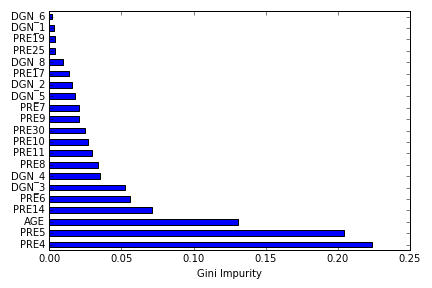
\includegraphics[width=0.5\textwidth]{../src/img/feature_importance.png}
\caption{Feature importance for all of the features after preprocessing.}
\label{fig:feature-importance}
\end{figure}

\subsection{Classifiers}
\label{subsec:classifiers}
Four classifiers were chosen for use on the dataset. The four classifiers used are Random Forests, Gradient Boosting, AdaBoost, and Extra Trees. The implementations of all four classifiers are taken directly from the scikit-learn library \cite{pedregosa2011scikit}. All of these methods are known as ensemble methods. Ensemble methods compose together multiple weak learners to produce a single strong classifier. In this paper, all of the algorithms used are also tree based (although this is not necessarily the case with Gradient Boosting and AdaBoost). This means that for each classifier the base learner is a decision tree.

Random forests \cite{breiman2001random} are perhaps the simplest method of the four. Random forests are simply a collection of $n$ decision trees which are individually trained on the data. The ``random'' in the name comes from the fact that each tree is trained on both a random sample of the dataset (tree bagging) and also on a random subset of the features (feature bagging). The decision tree weak learners typically overfit to the data. However because the results all trees are averaged over the resulting classification the overall variance in the final model is significantly reduced. The random element for both training instances and features is used to prevent many highly correlated trees from occurring which should reduce overfitting. 

Extremely Randomized trees \cite{geurts2006extremely} (also called Extra Trees) takes the randomisation aspect of random forests one step further. Both bagging and random features are used, but additionally a random split for each feature in the subset of features is chosen instead of the just computing the optimal feature and split combination.

The AdaBoost algorithm \cite{freund1997decision} is a generalised method from combining the performance of many weak learners. AdaBoost stands for ``adaptive boosting'' and boosting is a core component in the training stage. AdaBoost works by first fitting a weak learner to the training dataset and classifying each instance. The error in the classification can be used to re-weight each example in the dataset. This means that misclassified samples are then more likely to be classified correctly in future iterations. Likewise, instances that are correctly classifier can be weighted much lower, as they are easier to correctly identify. Thus AdaBoost can be seen as an additive method in that each tree is built on the error of the previous one. Adaboost does not necessarily have to be used with decision trees, but in this paper we only consider decision tree based AdaBoost.

Gradient Boosting Machines \cite{natekin2013gradient} also use a boosting based approach to learning. Like AdaBoost they are an additive method that iteratively fits a collection of weak learners. Where the two differ is in the way that instances are ``weighted''. The weighting function in AdaBoost can be seen as a special type of loss function. The gradient of a differentiable loss function can be use to steer the search towards the optimum decision function. In gradient boosting machines the new function added to the mix is the one which is the closest to parallel with the negative gradient of the observed data.

These algorithms were chosen to showcase a broad range of different ensemble algorithms. Ensemble methods often outperform a single strong learner due to the diversity present in the model. All of the models are also decision tree based which work well with a mixture of continuous and discrete values like those present in our dataset. 

Two common techniques used in training ensemble algorithms are bagging and boosting. This paper compares two algorithms based on boosting (AdaBoost and Gradient Boosting) and two based on bagging (Random Forests and Extra Trees). These seem like good candidates based on the dataset for two reasons: 1) bagging can be used address the imbalance in the dataset by equally resampling each of the datasets and 2) there doesn't seem to be a clear separation between classes in the dataset which potentially makes boosting a good technique as it should help to push the algorithm towards classify the difficult examples it's it misses.

\subsection{Hyperparameters \& Tuning}
\label{subsec:tuning}

Before all experiments were carried out on the dataset, the hyper-parameters of each classifier were tuned to hopefully achieve optimum performance. The values and number hyper-parameters are dependant both on the implementation of the classifier and the dataset itself. If there is more than one hyper-parameter for a classifier (as is the case with all classifiers used here) then ideally combinations of all hyper-parameters should be explored. Sadly, this means that the space of potential hyper-parameters explodes with the number of hyper-parameters increases.

Due to the relatively small size of the dataset, the space of potential parameters for each classifier is explored using a grid search. In a grid search, all a selection of hyper-parameter values are explicitly enumerated. Each potential value for a hyper-parameter is tested in combination with every other hyper-parameter value. The speed of the grid search is bearable due to the classifier being relatively quick to train on this small dataset. The performance of a set of parameters was evaluated using stratified $k$-fold cross validation with ROC AUC as the scoring metric.

For Random Forests a grid search was performed over the tree parameters \textit{max\_depth}, \textit{max\_features}, \textit{min\_samples\_split} and \textit{min\_samples\_leaf}. \textit{max\_depth} and \textit{max\_features} were trained over the range 2 - 20 in steps of 3. \textit{min\_samples\_split} and \textit{min\_samples\_leaf} were trained over all values in the range 1 - 5. The number of trees used was fixed to 50 during this search. This is because a small number of trees will be quick to train (and hence the search will complete faster). Generally speaking the performance of the forest should improve as the number of trees increases, so this can be trained afterwards.

The results of tuning the tree parameters showed that \textit{min\_samples\_split} and \textit{min\_samples\_leaf} should be set to 1. This seems logical due to the small number of positive samples. \textit{max\_depth}, \textit{max\_features} were optimised as 16 and 5 respectively. These seem reasonable given the low number of predictive features and the fact that trees in random forests should typically overfit (hence the large maximum depth). After this trial another grid search was performed to find the optimum number of trees over the range 50 - 500 in steps of 50. This suggested that 100 trees should be used. 

The training procedure for Extremely Random Trees was identical to Random Forests with the results being similar. After tuning 200 trees were used and \textit{max\_features} was set to 16 and \textit{max\_depth} set to 19.

Adaboost was tuned by fixing the maximum depth of the decision tree and performing a grid search over the number of trees (50 - 1000 in steps of 50) and the learning rate (with values 0.1, 0.5, 0.01, and 0.005) together. This was repeated for multiple values of the maximum depth (tested with values 2, 4, and 6). After tuning 400 trees were used with a \textit{learning\_rate} of 0.5 and \textit{max\_depth} of 4.

Gradient Boosting has many parameters that need to be explored, many of which can interact with one another and tuning in the wrong order can lead to poor results. The number of parameters can also be awkward to train due to the speed of training. The tuning procedure for gradient boosting was therefore as follows:

\begin{itemize}
	\item Fix all of the parameters to be reasonable initial guesses and fix the learning rate to be quite high (0.1).
	\item Find the optimum number of estimators for the given leaning rate (searched over the range 20 - 150 in steps of 10).
	\item Tune the tree based parameters \textit{max\_depth} and \textit{min\_samples\_split} (searched over the ranges 5-16 in steps of 2 and 1-20 in steps of 3 respectively).
	\item Tune \textit{max\_features} (5-20 in steps of 2)
	\item Tune the subsample ratio (values: 0.6, 0.7, 0.75, 0.8, 0.85, and 0.9).
	\item Finally using all previously tuned parameters increase the number of estimators while simultaneously decreasing the learning rate.
\end{itemize}

The final values for the tuned parameters used are shown in table \ref{table:gb-parameters}.

\begin{table}
\centering
\caption{Tuned Parameters for the Gradient Boosting Classifier}
\begin{tabular}{|l|l|}
\hline
\textbf{Parameter}                &       \textbf{Value}    \\
\hline
learning\_rate            &      0.01 \\ \hline
max\_depth                &         9 \\ \hline
max\_features             &        11 \\ \hline
min\_samples\_leaf         &         1 \\ \hline
min\_samples\_split        &         7 \\ \hline
n\_estimators             &      1000 \\ \hline
subsample                &       0.8 \\ \hline
\end{tabular}
\label{table:gb-parameters}

\end{table}


\section{Results}
\label{sec:results}

\subsection{Performance Evaluation}
\label{subsec:performance}

Each classifier in section \ref{subsec:classifiers} was trained using stratified 5-fold cross validation. Stratification was performed to ensure that there was a representative sample of positive classes in each fold. For all classifiers cross validation was repeated ten times, each with a new set of folds to ensure consistent results.

Figure \ref{fig:roc-cv} shows the mean ROC curve and mean AUC for each of the classifier after cross validation. The performance of each classifier appears to be very similar. Notably the ROC curve for each type of classifier is shifted to the right of the graph, suggesting that they all exhibit a low recall rate.

Table \ref{table:f-scores} and figure \ref{fig:f2-score} confirm this indication. Table \ref{table:f-scores} shows the F measure with a $\beta$ parameter of 1, 2, and 0.5. Figure \ref{fig:f2-score} shows a bar chart of the F2 scores in table \ref{table:f-scores}. The performance of all classifiers measured with the F2 score (which weights recall more highly than precision) is much lower in comparison to the F0.5 and F1 scores. This further confirms that all classifiers have a problem with recall.

\begin{table}
\caption{Mean F1, F2 and F0.5 scores for all four classifiers over 10 rounds of 5-fold cross validation.}
\label{table:f-scores}
\begin{tabular}{lrrrr}
{} &  RandomForest &  ExtraTrees &  GradientBoost &  AdaBoost \\
\hline
F1   &      0.601006 &    0.606542 &       0.623161 &  0.607031 \\
F2   &      0.522676 &    0.546392 &       0.567522 &  0.549125 \\
F0.5 &      0.715848 &    0.688120 &       0.700784 &  0.683489 \\
\end{tabular}

\end{table}

\begin{figure}[!t]
\centering
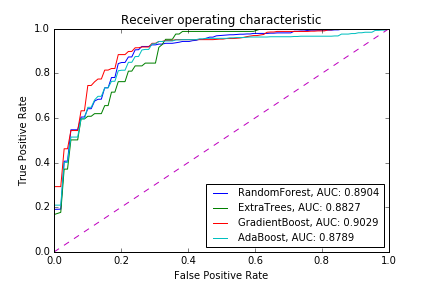
\includegraphics[width=0.5\textwidth]{../src/img/roc_cv.png}
\caption{Mean ROC curves and the mean AUC for all four classifiers over 10 rounds of 5-fold cross validation. All four classifiers perform similarly, with Extra Trees producing the best AUC. All four curves are slightly skewed towards the right of the plot, suggestive of poor recall. The F2 score (table \ref{table:f-scores} and figure \ref{fig:f2-score} confirms this.}
\label{fig:roc-cv}
\end{figure}

\begin{figure}[!t]
\centering
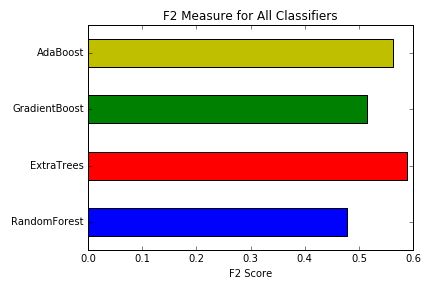
\includegraphics[width=0.5\textwidth]{../src/img/f2_score.png}
\caption{Bar chart showing the F2 score for all classifiers taken from table \ref{table:f-scores}.}
\label{fig:f2-score}
\end{figure}

\subsection{Feature Engineering}
In addition to the preprocessing steps outlined in \ref{subsec:dataset} several combinations of new features were generated from the existing predictors. Firstly, as a large portion of the features are binary, a set of new features were created based on logical binary operators. The creation of the binary features is as follows: all pairs of binary features are enumerated. From each pair three new features are created by combining the pair using logical OR, AND and XOR.

Figure \ref{fig:roc-binary-features} shows the ROC curves for the same dataset but with the additional binary features. appended. Table \ref{table:f-scores-binary} shows the corresponding F-scores for each classifier. From these results it is easy to see that all of the classifiers appear to perform worse with the new features. This may be due to their already limited contribution and that fact that the additional dimensionality is hindering progress.

\begin{figure}[!t]
\centering
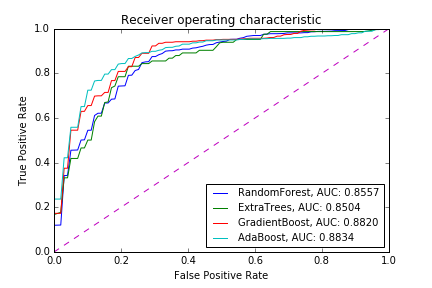
\includegraphics[width=0.5\textwidth]{../src/img/roc_binary_features.png}
\caption{ROC curves for each of the classifiers with the additional binary features. Performance is notably worse compared to the initial run.}
\label{fig:roc-binary-features}
\end{figure}


\begin{table}
\caption{F scores for the dataset including binary features}
\begin{tabular}{lrrrr}
{} &  RandomForest &  ExtraTrees &  GradientBoost &  AdaBoost \\
\hline
F1   &      0.543811 &    0.560718 &       0.612539 &  0.646753 \\
F2   &      0.465938 &    0.489906 &       0.547107 &  0.591129 \\
F0.5 &      0.662682 &    0.660713 &       0.705097 &  0.721499 \\
\end{tabular}
\label{table:f-scores-binary}	
\end{table}


The second modification to the original dataset is to create a couple of new features called FER and OBS. FER is the FEV1/FVC ratio which is spirometry measurement defined as $(FEV1/FVC) \cdot 100$ \cite{patient2016spirometry}. It is interpreted as the percentage of FVC expelled in the first second of a forced expiration. A ratio value below <70\% can be suggestive of an obstructive disease. Using this information another feature (OBS) is generated from the ratio. OBS is a binary feature with value 1 when a patient has a ratio <70\%.

From figure \ref{fig:roc-spiro-features} it can be seen that their is a slight improvement over the original ROC AUC scores using these additional spirometry features. This is backed up by plotting the feature importance obtained from training a random forest on the dataset (see \ref{fig:feature-importance}). The two new features, particularly the FER feature are providing useful training information. This seems sensible as the new features are just combinations of existing well performing features.

\begin{figure}[!t]
\centering
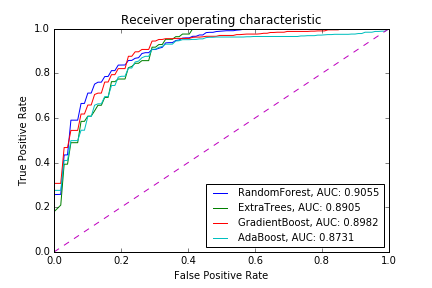
\includegraphics[width=0.5\textwidth]{../src/img/roc_spiro_features.png}
\caption{ROC curves for each of the classifiers with the spirometry features.}
\label{fig:roc-spiro-features}
\end{figure}

\begin{figure}[!t]
\centering
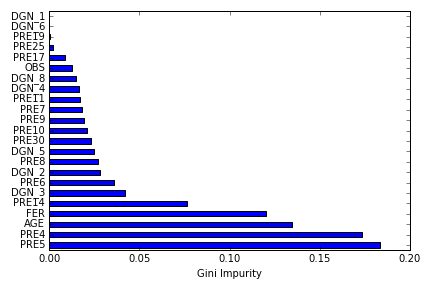
\includegraphics[width=0.5\textwidth]{../src/img/importance_spiro_features.png}
\caption{Variable importance for each of the features with the spirometry features included.}
\label{fig:importance-spiro-features}
\end{figure}

\begin{table}
\caption{F scores for the dataset including spirometry features}
\begin{tabular}{lrrrr}
{} &  RandomForest &  ExtraTrees &  GradientBoost &  AdaBoost \\
\hline
F1   &      0.566669 &    0.617225 &       0.600845 &  0.614050 \\
F2   &      0.483774 &    0.549281 &       0.538619 &  0.561441 \\
F0.5 &      0.699297 &    0.715047 &       0.688793 &  0.683218 \\
\end{tabular}
\end{table}

Motivated by the results of the previous test, a selection of new features were created from all order 2 polynomial combinations of the two best predictors: PRE4 and PRE5. This means that the new features are of the form $a^2$, $ab$, $b^2$ where $a$ and $b$ are PRE4 and PRE5 respectively. 

This polynomial combination led to the best in the feature engineering results across all classifiers under cross validation. Figure \ref{fig:roc-poly-features} shows the ROC curves with the additional features included. The F-scores for each classifier are show in table \ref{table:f-scores-poly}. The contribution of the new features can be seen in the variable importance plot (figure \ref{fig:importance-poly-features}).

\begin{figure}[!t]
\centering
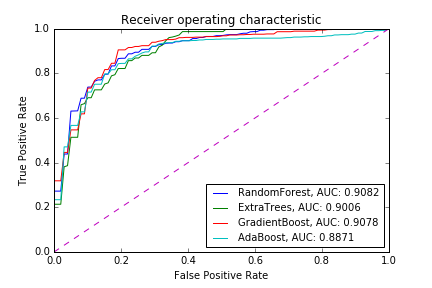
\includegraphics[width=0.5\textwidth]{../src/img/roc_poly_features.png}
\caption{ROC curves for each of the classifiers with the polynomial combination features.}
\label{fig:roc-poly-features}
\end{figure}

\begin{figure}[!t]
\centering
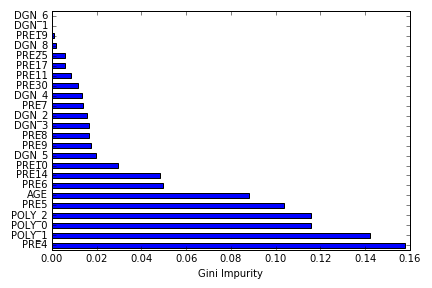
\includegraphics[width=0.5\textwidth]{../src/img/importance_poly_features.png}
\caption{Variable importance for each of the features with the polynomial combination features included.}
\label{fig:importance-poly-features}
\end{figure}

\begin{table}
\caption{F scores for the dataset including polynomial combination features}
\begin{tabular}{lrrrr}
{} &  RandomForest &  ExtraTrees &  GradientBoost &  AdaBoost \\
\hline
F1   &      0.604371 &    0.634325 &       0.615442 &  0.662434 \\
F2   &      0.517592 &    0.563459 &       0.560582 &  0.613066 \\
F0.5 &      0.736327 &    0.732681 &       0.690843 &  0.726515 \\
\end{tabular}

\label{table:f-scores-poly}	
\end{table}

\subsection{Dataset Balancing}
\label{subsec:dataset-balancing}
As mentioned in section \ref{subsec:dataset} the thoracic surgery dataset is class imbalanced with only 28\% of the dataset being of the positive class. One technique to combat class imbalance is to resample the dataset to put more emphasis on the known positive examples. A popular technique for resampling data is SMOTE \cite{chawla2002smote}. SMOTE rebalances a dataset by creating new synthetic training to balance out the majority class. SMOTE is typically combined with under-sampling of the majority class to produce a final dataset that is re-weighted in favour of the minority class. 

The results for the classifiers in part \ref{subsec:performance} shows that they have lower recall than precision. Rebalancing the dataset should show a decrease in precision and an increase in recall rate. This can be desirable in a dataset such as this where recall may be more important than precision. It is probably more desirable overestimate the number people who are likely to die from surgery than to achieve better precision.

SMOTE datasets cannot be validated using conventional k-fold cross validation. This is because the testing fold would contain synthetically generated training examples which are obviously not representative of the ground truth. Instead, in order to achieve a representative sample of performance, ``Monte Carlo'' cross-validation \cite{dubitzky2007fundamentals} is used. Before a any resampling is applied, the data set is randomly split into a training and testing set. The split is stratified according to the class labels. All reported experiments use and 80/20 split. Resampling is then applied to the training dataset only, with the testing set remaining untouched. This process is then repeated for the desired number of iterations and the resulting performance measures are averaged. In all experiments the number of iterations performed was 50.  

Figure \ref{fig:roc-smote} shows ROC curve and mean AUC scores for each of the classifiers using SMOTE with a resampling ratio of 0.8. Table \ref{table:f-score-smote} shows the F1, F2, and F0.5 scores for each of the classifiers. Comparing this table to the results of \ref{table:f-scores} shows a clear difference in the F2 score. Recall weighted performance is now better both than F1 and F0.5. This improvement comes at the cost of a decrease in both the AUC and F0.5 measures. Increasing the oversampling ratio or under-sampling the majority class accentuates this effect.

\begin{figure}[!t]
\centering
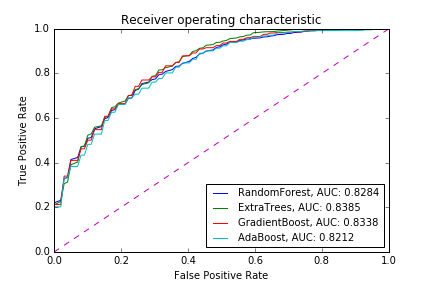
\includegraphics[width=0.5\textwidth]{../src/img/roc_smote.png}
\caption{ROC curves for all four classifiers with SMOTE oversampling with a ratio of 0.8. Each curve represents the average over 50 iterations of Monte Carlo validation. The ROC curves for all classifiers are less skewed compared to figure \ref{fig:roc-cv}.}
\label{fig:roc-smote}
\end{figure}

\begin{table}
\caption{Mean F1, F2 and F0.5 scores for all classifiers after monte carlo cross validation with SMOTE resampling with a ratio of 0.8}
\begin{tabular}{lrrrr}
{} &  RandomForest &  ExtraTrees &  GradientBoost &  AdaBoost \\
\hline
F1   &      0.614570 &    0.613840 &       0.615768 &  0.611035 \\
F2   &      0.648492 &    0.650097 &       0.648949 &  0.643250 \\
F0.5 &      0.587619 &    0.585145 &       0.589706 &  0.586983 \\
\end{tabular}
\label{table:f-score-smote}
\end{table}

\section{Discussion}
\label{sec:discussion}
The experiments in section \ref{sec:results} have shown a variety of different approaches to predicting surgery survival with ensemble methods. Some of the best performance was achieved using the just the basic preprocessing steps outlined in section \ref{subsec:dataset}.

Looking at the initial performance evaluation (figure \ref{fig:roc-cv}) it can be seen that all classifiers performed reasonable similarly with Gradient Boosting narrowly coming out ahead. The weakest performer was AdaBoost. Looking at the F-scores for each of the classifiers (table \ref{table:f-scores}) is more informative. All classifiers can be seen to perform comparable. Each performed weaker under the F2 measure which weights recall more highly than precision. It is the higher recall rate which is primarily driving the improvement of Gradient Boosting over the other classifiers in this trial.

Motivated by this baseline evaluation, this paper explored alternative feature representations through ``feature engineering''. The first attempt was to create combinations of binary features from the existing dataset. This actually lead to worse results compared to the original preprocessing steps. None of the new binary features significantly contributed new information for the algorithm to work with. This probably meant that the increase in dimensionality out weighed any small gains delivered by the new representation. Each tree in the ensembles will only look at a limited number of features, so adding lots of redundant features is only likely to decrease performance while increasing training time. Note that an attempt was made to reduce the number of features by discarding the $n$ weakest features using both variable importance and PCA, but neither method improved the results of this test.

The second feature engineering experiment was to a couple of features generated from spirometry theory. Both the FER and OBS feature suggested are directly derived from the existing predictors in the dataset. The bar chart in figure \ref{fig:importance-spiro-features} shows that these features do appear to contribute some additional information for the classifiers to work with. This is reflected in the AUC scores and the corresponding F-scores. The result for AUC is nearly identical between Gradient Boosting, Extra-Trees, and Random forests. The most successful (by a tiny margin) showed that Random forests performed the best in terms in AUC but this was only due to high precision. The F2 and F1 score are both much reduced in in the Random Forest trial. With these new features the best candidate appears to be Extra-Trees which has an improvement across all three F-scores.

The third experiment involving feature engineering was to create a new batch of features by creating polynomial combinations of the features PRE4 and PRE5 which were shown to be the strongest predictors in figure \ref{fig:feature-importance}. This lead to the best AUC scores out of all the trails with three out of the four classifiers pushing into the 0.9 range. The variable importance plot (\ref{fig:importance-poly-features}) shows that many of the polynomial features are the most successful contributors. The F-scores reflect this result and show higher scores across the board. By far the biggest increase was in terms of precision. In particular, AdaBoost faired much better with polynomial features.

Finally an experiment was carried looking at improving the performance by resampling the dataset using SMOTE. While random forests and extra-trees already carry out bagging which already balances the dataset during training, this method could of potentially helped the performance of the boosting classifiers. Figure \ref{fig:roc-smote} shows a marked decrease in performance across all classifiers. This is probably due to the synthetic examples not realistically reflecting the distribution of positive examples in the dataset. What is more interesting is the fact that the F2 scores for each classifier are improved by applying SMOTE but the precision is dramatically hindered. This is could be due to the synthetic examples ``expanding'' the region around positive examples which the algorithm considers to be positive. This is probably not representative of the true decision boundary, but has the effect of increasing recall as more examples are likely to land with the expanded positive region. While this test resulted in much worse performance it could still be of interest. In predicting thoracic surgery survival it is more desirable to have high recall than high precision.


\section{Conclusions}
\label{sec:conclusions}
In conclusion this paper examined the effect of four different ensemble methods on a variety of engineered features. The effect of resampling the dataset was also explored. The final classifier used on the unused testing data for submission was trained using both the additional polynomial and spirometry features. This lead to best performance with the {} classifier. This classifier had a final AUC after cross validation of {}.

While this is one of the best AUC scores achieved across all experiments there is clearly some room from improvement. One area of improvement worth exploring would be to look at more automated methods of feature selection. One such method could be recursive feature elimination in conjunction with a model that estimates feature relevance (such as random forests). Alternatively a non-linear dimensionality reduction technique could be used to find projections of the feature space onto a lower dimensional embedding. This could be particular beneficial in the case of the binary features where the feature space is relatively much larger. 

Another avenue for exploration would be to look at a different branch of algorithms. For example a penalised SVM could be experimented with. The original authors of \cite{zikeba2014boosted} propose a boosted SVM which performs reasonable well on the expanded dataset. Any alternative classifier will probably benefit from some from of bagging or resampling more than the ensemble methods.

The experiments in this paper show that any further predictive progress appears to be hindered by the low recall rate. This is a common trade-off in machine learning. Implementing this system in the real world would most likely require favouring a lower F0.5 score for a higher F2 for safety reasons. Any progress beyond the AUC achieved in this paper is likely to require a combination of further creative feature engineering and a good mix of bagging/resampling.

\bibliographystyle{IEEEtran}
\bibliography{references}

% needed in second column of first page if using \IEEEpubid
%\IEEEpubidadjcol

% An example of a floating figure using the graphicx package.
% Note that \label must occur AFTER (or within) \caption.
% For figures, \caption should occur after the \includegraphics.
% Note that IEEEtran v1.7 and later has special internal code that
% is designed to preserve the operation of \label within \caption
% even when the captionsoff option is in effect. However, because
% of issues like this, it may be the safest practice to put all your
% \label just after \caption rather than within \caption{}.
%
% Reminder: the "draftcls" or "draftclsnofoot", not "draft", class
% option should be used if it is desired that the figures are to be
% displayed while in draft mode.
%
%\begin{figure}[!t]
%\centering
%\includegraphics[width=2.5in]{myfigure}
% where an .eps filename suffix will be assumed under latex, 
% and a .pdf suffix will be assumed for pdflatex; or what has been declared
% via \DeclareGraphicsExtensions.
%\caption{Simulation Results}
%\label{fig_sim}
%\end{figure}

% Note that IEEE typically puts floats only at the top, even when this
% results in a large percentage of a column being occupied by floats.


% An example of a double column floating figure using two subfigures.
% (The subfig.sty package must be loaded for this to work.)
% The subfigure \label commands are set within each subfloat command, the
% \label for the overall figure must come after \caption.
% \hfil must be used as a separator to get equal spacing.
% The subfigure.sty package works much the same way, except \subfigure is
% used instead of \subfloat.
%
%\begin{figure*}[!t]
%\centerline{\subfloat[Case I]\includegraphics[width=2.5in]{subfigcase1}%
%\label{fig_first_case}}
%\hfil
%\subfloat[Case II]{\includegraphics[width=2.5in]{subfigcase2}%
%\label{fig_second_case}}}
%\caption{Simulation results}
%\label{fig_sim}
%\end{figure*}
%
% Note that often IEEE papers with subfigures do not employ subfigure
% captions (using the optional argument to \subfloat), but instead will
% reference/describe all of them (a), (b), etc., within the main caption.


% An example of a floating table. Note that, for IEEE style tables, the 
% \caption command should come BEFORE the table. Table text will default to
% \footnotesize as IEEE normally uses this smaller font for tables.
% The \label must come after \caption as always.
%
%\begin{table}[!t]
%% increase table row spacing, adjust to taste
%\renewcommand{\arraystretch}{1.3}
% if using array.sty, it might be a good idea to tweak the value of
% \extrarowheight as needed to properly center the text within the cells
%\caption{An Example of a Table}
%\label{table_example}
%\centering
%% Some packages, such as MDW tools, offer better commands for making tables
%% than the plain LaTeX2e tabular which is used here.
%\begin{tabular}{|c||c|}
%\hline
%One & Two\\
%\hline
%Three & Four\\
%\hline
%\end{tabular}
%\end{table}


% Note that IEEE does not put floats in the very first column - or typically
% anywhere on the first page for that matter. Also, in-text middle ("here")
% positioning is not used. Most IEEE journals use top floats exclusively.
% Note that, LaTeX2e, unlike IEEE journals, places footnotes above bottom
% floats. This can be corrected via the \fnbelowfloat command of the
% stfloats package.







% if have a single appendix:
%\appendix[Proof of the Zonklar Equations]
% or
%\appendix  % for no appendix heading
% do not use \section anymore after \appendix, only \section*
% is possibly needed

% use appendices with more than one appendix
% then use \section to start each appendix
% you must declare a \section before using any
% \subsection or using \label (\appendices by itself
% starts a section numbered zero.)
%

\clearpage
\onecolumn
\appendices

\section{Third Party Libraries}
The code use to produce the results in the paper rely upon a number of different third party libraries. The libraries used and the relevant version of each is show in the table below. lease note that the \textit{UnbalancedData} library is not currently directly available through \textit{pip} by default and so must be installed directly from the GitHub repository using the following command:

\begin{lstlisting}
	pip install git+https://github.com/fmfn/UnbalancedDataset
\end{lstlisting}

\begin{table}[H]
\centering
\caption{Third party libraries and the accompanying versions used in all the following code samples.}
\label{my-label}
\begin{tabular}{|l|l|}
\hline
\textbf{Name}     & \textbf{Version} \\ \hline
pandas            & 0.18.0           \\ \hline
sklearn           & 0.17.1           \\ \hline
UnbalancedDataset & 0.1              \\ \hline
matplotlib        & 1.5.1            \\ \hline
numpy             & 1.11.0           \\ \hline
scipy             & 0.17.0           \\ \hline
\end{tabular}
\end{table}

\section{Python Script for Final Classifier}
\label{appendix:final-classifier}
This appendix contains the python script for creating the final classifier used to make the predictions on the test dataset for this assignment. This will save a CSV file in the data folder called \textit{submission.csv}.

\lstinputlisting[language=Python]{../src/classify.py}

\section{IPython Notebook and Additional Python Modules for Analysis, Training and Tuning}
This listing shows the contents of the analysis IPython notebook as a python script. For a better formatted version of this code install IPython and open the Analysis.ipynb file provided with the assignment submission. This IPython notebook contains all of the code for analysing the data, tuning the algorithms, and performing both stratified k-fold and Mote Carlo cross validation. Two additional modules (\textit{pipeline} and \textit{roc\_analysis}) are also provided as listing as the end of this section.

\lstinputlisting[language=Python]{../src/analysis.py}

\subsection{ROC Analysis Module}
\lstinputlisting[language=Python]{../src/roc_analysis.py}

\subsection{Pipeline Module}
\lstinputlisting[language=Python]{../src/pipeline.py}

\section{Final Predictions}
This listing shows the final submission CSV file generated from the code in \ref{appendix:final-classifier}.  

\lstinputlisting[language=Python]{../data/submission.csv}


% use section* for acknowledgement
%\section*{Acknowledgment}
%
%
%The authors would like to thank...


% Can use something like this to put references on a page
% by themselves when using endfloat and the captionsoff option.
\ifCLASSOPTIONcaptionsoff
  \newpage
\fi



% trigger a \newpage just before the given reference
% number - used to balance the columns on the last page
% adjust value as needed - may need to be readjusted if
% the document is modified later
%\IEEEtriggeratref{8}
% The "triggered" command can be changed if desired:
%\IEEEtriggercmd{\enlargethispage{-5in}}

% references section

% can use a bibliography generated by BibTeX as a .bbl file
% BibTeX documentation can be easily obtained at:
% http://www.ctan.org/tex-archive/biblio/bibtex/contrib/doc/
% The IEEEtran BibTeX style support page is at:
% http://www.michaelshell.org/tex/ieeetran/bibtex/
%\bibliographystyle{IEEEtran}
% argument is your BibTeX string definitions and bibliography database(s)
%\bibliography{IEEEabrv,../bib/paper}
%
% <OR> manually copy in the resultant .bbl file
% set second argument of \begin to the number of references
% (used to reserve space for the reference number labels box)

%\begin{thebibliography}{1}
%
%\bibitem{IEEEhowto:kopka}
%H.~Kopka and P.~W. Daly, \emph{A Guide to \LaTeX}, 3rd~ed.\hskip 1em plus
%  0.5em minus 0.4em\relax Harlow, England: Addison-Wesley, 1999.
%
%\end{thebibliography}

% biography section
% 
% If you have an EPS/PDF photo (graphicx package needed) extra braces are
% needed around the contents of the optional argument to biography to prevent
% the LaTeX parser from getting confused when it sees the complicated
% \includegraphics command within an optional argument. (You could create
% your own custom macro containing the \includegraphics command to make things
% simpler here.)
%\begin{biography}[{\includegraphics[width=1in,height=1.25in,clip,keepaspectratio]{mshell}}]{Michael Shell}
% or if you just want to reserve a space for a photo:

%\begin{IEEEbiography}[{\includegraphics[width=1in,height=1.25in,clip,keepaspectratio]{picture}}]{John Doe}
%\blindtext
%\end{IEEEbiography}

% You can push biographies down or up by placing
% a \vfill before or after them. The appropriate
% use of \vfill depends on what kind of text is
% on the last page and whether or not the columns
% are being equalized.

%\vfill

% Can be used to pull up biographies so that the bottom of the last one
% is flush with the other column.
%\enlargethispage{-5in}



% that's all folks
\end{document}


